\chapter{Development}

\section{Cache}
\dots

\section{Motion capture}
\begin{center}
	\begin{figure}[ht!]
		\makebox[\textwidth]{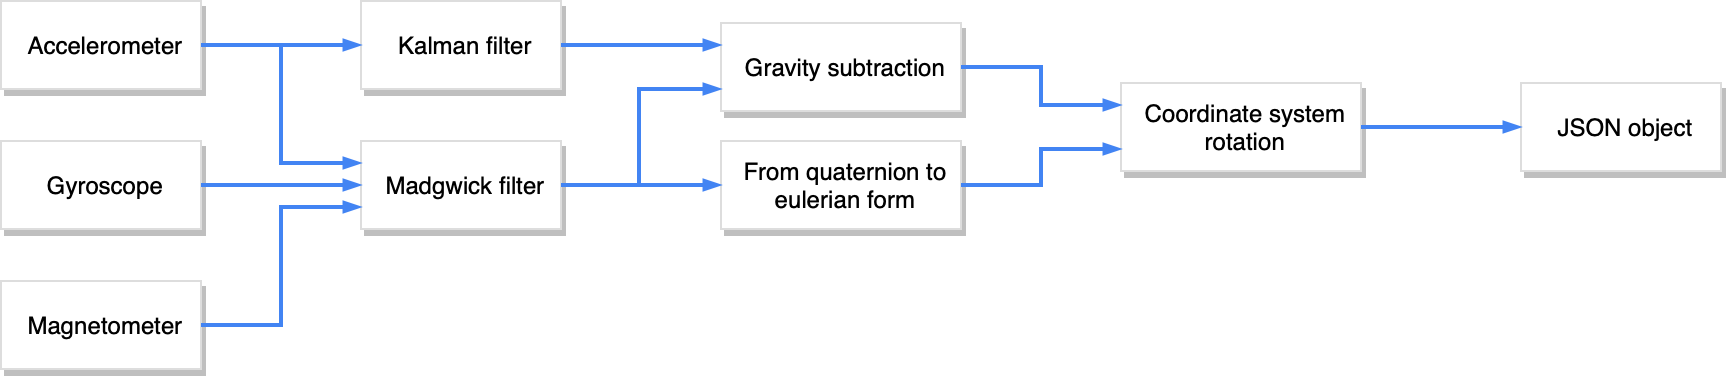
\includegraphics[width=0.5\paperwidth]{img/data_fusion.png}}
		\caption{Data fusion schema.}
	\end{figure}
\end{center}
Previously, the data collected were:
\begin{itemize}
	\item yaw, pitch and roll angles;
	\item acceleration with components in spherical coordinates system;
	\item raw gyroscope data;
	\item a velocity approximation.
\end{itemize}
\bigbreak

The aim was to detect \textit{discriminating features among different playing patterns}, collecting and analyzing data from the sensors; the analysis followed the flow in the data fusion schema, except for the velocity approximation.
\bigbreak

The velocity approximation, calculated by the \textit{Velocimeter} [CITE] was excluded because of its practical difficulty in obtaining realistic values using only inertial sensors, where measurement errors are unavoidable, especially for miniature MEMS sensors. Direct integration of acceleration often causes unrealistic drifts in velocity, due to errors propagation; furthermore, measured acceleration not only carries random noise, but also presents with offset caused by temperature drift, resulting in estimation errors accumulated by integration process. [CITE \href{http://www.chrobotics.com/library/accel-position-velocity}{here} and papers], that results in low accuracy.
\bigbreak

IMAGE OF THE SQUARE WAVE\\
tessellation of the truck's tyre
\bigbreak

The first analysis dealt with raw accelerometer data, but the noisiness of the signal and the lack of gravity removal have induced to desist. Nevertheless, more often than not the main waveform was recognizable, especially for movements with strong accelerations (that simply increase the signal-to-noise ratio).
\bigbreak

The analysis moved to Kalman-filtered data, which revealed much cleaner, but still included gravity; thus it was necessary a more complex training data collection, due to the lack of orientation invariance (in order to obtain such invariance it would have been necessary to collect every pattern with the toy rotated in any possible angle).

Nevertheless, gravity-free acceleration data were computed by the device (with the help of Madgwick's fusion algorithm) and sent to the server but not stored in the database, only used for the 3D visual representation, both in training and session recording phase. It was decided to keep such data and analyze it to see if it was reliable over time.
\bigbreak

Some testing showed quickly that there was an error in the yaw angle calculation: the more the toy was rotated (regardless of the axis), the more the yaw diverged. Such error was initially imputed to the Madgwick algorithm implementation, more precisely to the convergence of its error-correction gradient descent algorithm. Unfortunately, different algorithm implementations and different values of the algorithm's gain parameter (the magnitude $\beta$ of the gyroscope measurement error\footnote{Increasing $\beta$ leads to faster bias corrections and higher sensitiveness to lateral accelerations.} [CITE]) have no given better results over time, and worse, sometimes ghost accelerations were found.
\bigbreak

IMAGE OF DIFFERENT ACCELERATIONS FOR THE SAME\\ PATTERN
\bigbreak

During the tests, it was noticed that recordings of the same pattern with different device orientations didn't split the acceleration differently among axes, revealing that the reference system was integral with the Earth's center instead of the device's sensor center. To align it back, the acceleration vector has been rotated using a 3D rotation matrix. The 3 rotation angles are given by the Madgwick algorithm.
\bigbreak

A \textit{yaw} is a CCW rotation of $\alpha$ on the $z$-axis. The rotation matrix is
\[
	R_z(\alpha) =
	\begin{pmatrix}
		\cos\alpha & -\sin\alpha & 0 \\
		\sin\alpha & \cos\alpha & 0 \\
		0 & 0 & 1
	\end{pmatrix}
\]
Note that the upper left values compose a 2D rotation matrix, and the coordinates on the third dimension (around whom the rotation happens) are left unchanged. The same applies to the other two matrices, but with the second and the first dimension.
\bigbreak

A \textit{pitch} is a CCW rotation of $\beta$ on the $y$-axis. The rotation matrix is
\[
	R_y(\beta) =
	\begin{pmatrix}
		\cos\beta & 0 & \sin\beta \\
		0 & 1 & 0 \\
		-sin\beta & 0 & \cos\beta
	\end{pmatrix}
\]

A \textit{roll} is a CCW rotation of $\gamma$ on the $x$-axis. The rotation matrix is
\[
	R_x(\gamma) =
	\begin{pmatrix}
		1 & 0 & 0 \\
		0 & \cos\gamma & -\sin\gamma \\
		0 & sin\gamma & \cos\gamma
	\end{pmatrix}
\]
\begin{gather*}
	R(\alpha, \beta, \gamma) = R_z(\alpha) R_y(\beta) R_x(\gamma) = \\
	\begin{pmatrix}
		\cos\alpha \cos\beta & \cos\alpha \sin\beta \sin\gamma - \sin\alpha \cos\gamma & \cos\alpha \sin\beta \cos\gamma + \sin\alpha \sin\gamma \\
		\sin\alpha \cos\beta & \sin\alpha \sin\beta \sin\gamma + \cos\alpha \cos\gamma & \sin\alpha \sin\beta \cos\gamma - \cos\alpha \sin\gamma \\
		-\sin\beta & \cos\beta \sin\gamma & \cos\beta \cos\gamma
	\end{pmatrix}
\end{gather*}
It is important to note that $R(\alpha, \beta, \gamma)$ performs the roll first, then the pitch, and finally the yaw. If the order of these operations is changed, a different rotation matrix would result [CITE].
\bigbreak

Given an acceleration vector $\vec a$, the rotated one is $\vec a_r = R(\alpha, \beta, \gamma) \vec a$.
The matrix-vector multiplication doesn't need specific optimizations in the code because the dimensions at stake are too small for a meaningful speed or space improvement, and however the C++ code is compiled by \texttt{GCC} with the \texttt{-Os} flag, that includes the loop unrolling optimization [CITE].
\bigbreak

The coordinate system rotation solved both problems: the coordinate system was integral with the toy, and the yaw angle was calculated correctly.
\bigbreak

Once achieved a reliable gravity-filtered acceleration approximation, it was possible to perform some fine tuning. Magnetic and inertial sensors can be influenced by magnetic disturbance [CITE]. Madgwick's algorithm can remove interferences from Earth's frame (\textit{soft iron}) [CITE Madgwick] that cause errors in the measured direction of the Earth's magnetic field. \textit{Hard iron} distortions are produced by materials that exhibit a constant, additive field to the Earth's magnetic field [CITE \href{https://www.fierceelectronics.com/components/compensating-for-tilt-hard-iron-and-soft-iron-effects}{this}], and they can be removed through calibration [CITE my papers and from 42 to 45 in Madgwick's report]. The calibration has been performed by the SparkFun's Arduino library.

Unfortunately, there are non-constant interferences that still affect the sensors readings, such as the magnetic field generated by the current passing through the USB cable for charging the battery.
Its removal is much harder, because requires to analyze how much current is flowing through the cable, and the knowledge of the net magnetic field's shape, that depends on how the cable is placed around the sensor.
\bigbreak

IMAGE OF THE YAW AFFECTED BY THE BATTERY CHARGING.

\section{Delay in real-time data plotting}
\dots
